%!TEX root = ../main.tex

\newpage
\section*{Supplementary}

  \renewcommand{\thefigure}{S\arabic{figure}}
  \setcounter{figure}{0}

  \renewcommand{\thetable}{S\arabic{table}}
  \setcounter{table}{0}

  \begin{table}[H]
\centering
\small
\begin{tabular}{|c|c|c|c|c|}
\hline
\textbf{Step}                         & \textbf{Task}                   & \textbf{Module}                                   & \textbf{Parameter}           & \textbf{Value}   \\ \hline
\multirow{14}{*}{Sequence Processing} & \multirow{6}{*}{Demultiplexing} & \multirow{3}{*}{demultiplexing\_illumina\_single} & barcode\_column              & barcode-sequence \\
                                      &                                 &                                                   & rev\_comp\_barcodes          & false            \\
                                      &                                 &                                                   & rev\_comp\_mapping\_barcodes & false            \\ \cline{3-5}
                                      &                                 & \multirow{3}{*}{demultiplexing\_illumina\_paired} & barcode\_column              & barcode-sequence \\
                                      &                                 &                                                   & rev\_comp\_barcodes          & false            \\
                                      &                                 &                                                   & rev\_comp\_mapping\_barcodes & false            \\ \cline{2-5}
                                      & \multirow{8}{*}{Trimming}       & export\_visualization\_single                     & seq\_samplesize              & 10000            \\ \cline{3-5}
                                      &                                 & export\_visualization\_paired                     & seq\_samplesize              & 10000            \\ \cline{3-5}
                                      &                                 & \multirow{3}{*}{trimming\_single}                 & ncpus                        & 1                \\
                                      &                                 &                                                   & max\_ee                      & 2                \\
                                      &                                 &                                                   & trunc\_q                     & 2                \\ \cline{3-5}
                                      &                                 & \multirow{3}{*}{trimming\_paired}                 & ncpus                        & 1                \\
                                      &                                 &                                                   & max\_ee                      & 2                \\
                                      &                                 &                                                   & trunc\_q                     & 2                \\ \hline
\end{tabular}
\caption{The default parameters used in the Sequence Processing step of the \ac{micone} pipeline}
\label{tab:sp_parameters}
\end{table}

\begin{table}[H]
\centering
\small
\begin{tabular}{lllll}
\hline
\textbf{Step}                             & \textbf{Task}                                            & \textbf{Tool}                          & \textbf{Parameter}                     & \textbf{Value}                                                                                           \\ \hline
\multirow{17}{*}{Sequence Processing}     & \multirow{4}{*}{Bootstrap}                               & \multirow{3}{*}{resample}              & bootstraps                             & 1000                                                                                                     \\
                                          &                                                          &                                        & ncpus                                  & 1                                                                                                        \\
                                          &                                                          &                                        & filter\_flag                           & True                                                                                                     \\
                                          &                                                          & pvalue                                 & ncpus                                  & 1                                                                                                        \\ \cline{2-5}
                                          & \multirow{12}{*}{Correlation}                            & \multirow{2}{*}{sparcc}                & iterations                             & 50                                                                                                       \\
                                          &                                                          &                                        & ncpus                                  & 1                                                                                                        \\
                                          &                                                          & pearson                                & -                                      & -                                                                                                        \\
                                          &                                                          & spearman                               & -                                      & -                                                                                                        \\
                                          &                                                          & \multirow{5}{*}{spieceasi}             & method                                 & mb                                                                                                       \\
                                          &                                                          &                                        & ncpus                                  & 1                                                                                                        \\
                                          &                                                          &                                        & nreps                                  & 50                                                                                                       \\
                                          &                                                          &                                        & nlambda                                & 20                                                                                                       \\
                                          &                                                          &                                        & lambda\_min\_ratio                     & 1e-2                                                                                                     \\
                                          &                                                          & \multirow{2}{*}{mldm}                  & z\_mean                                & 1                                                                                                        \\
                                          &                                                          &                                        & max\_iteration                         & 1500                                                                                                     \\
                                          &                                                          & magma                                  & -                                      & -                                                                                                        \\ \cline{2-5}
                                          & Network                                                  & make\_network                          & -                                      & -                                                                                                        \\ \hline
\end{tabular}
\caption{The default parameters used in the various tools of the pipeline}
\label{tab:all_parameters}
\end{table}

\begin{table}[H]
\centering
\small
\begin{tabular}{lllll}
\hline
\textbf{Step}                             & \textbf{Task}                                            & \textbf{Tool}                          & \textbf{Parameter}                     & \textbf{Value}                                                                                           \\ \hline
\multirow{29}{*}{Denosing and Clustering} & \multicolumn{1}{c}{\multirow{9}{*}{Sequence Processing}} & \multirow{2}{*}{join\_reads}           & min\_overlap                           & 6                                                                                                        \\
                                          & \multicolumn{1}{c}{}                                     &                                        & perc\_max\_diff                        & 8                                                                                                        \\
                                          & \multicolumn{1}{c}{}                                     & \multirow{2}{*}{demultiplex\_illumina} & rev\_comp\_barcodes                    & False                                                                                                    \\
                                          & \multicolumn{1}{c}{}                                     &                                        & rev\_comp\_mapping\_barcodes           & False                                                                                                    \\
                                          & \multicolumn{1}{c}{}                                     & demultiplex\_454                       & -                                      & -                                                                                                        \\
                                          & \multicolumn{1}{c}{}                                     & \multirow{4}{*}{trim\_filter\_fixed}   & seq\_sample\_size                      & 10,000                                                                                                   \\
                                          & \multicolumn{1}{c}{}                                     &                                        & ncpus                                  & 1                                                                                                        \\
                                          & \multicolumn{1}{c}{}                                     &                                        & trunc\_q                               & 2                                                                                                        \\
                                          & \multicolumn{1}{c}{}                                     &                                        & max\_ee                                & 2                                                                                                        \\ \cline{2-5}
                                          & \multirow{3}{*}{Chimera Checking}                        & uchime                                 & -                                      & -                                                                                                        \\
                                          &                                                          & \multirow{2}{*}{remove\_bimera}        & ncpus                                  & 1                                                                                                        \\
                                          &                                                          &                                        & chimera\_method                        & consensus                                                                                                \\ \cline{2-5}
                                          & \multirow{17}{*}{Denoise Cluster}                        & \multirow{3}{*}{de\_novo}              & enable\_rev\_strand\_match             & True                                                                                                     \\
                                          &                                                          &                                        & suppress\_de\_novo\_chimera\_detection & True                                                                                                     \\
                                          &                                                          &                                        & ncpus                                  & 1                                                                                                        \\
                                          &                                                          & \multirow{4}{*}{closed\_reference}     & enable\_rev\_strand\_match             & True                                                                                                     \\
                                          &                                                          &                                        & suppress\_de\_novo\_chimera\_detection & True                                                                                                     \\
                                          &                                                          &                                        & ncpus                                  & 1                                                                                                        \\
                                          &                                                          &                                        & reference\_sequences                   & 97\_otus.fasta                                                                                           \\
                                          &                                                          & \multirow{5}{*}{open\_reference}       & enable\_rev\_strand\_match             & True                                                                                                     \\
                                          &                                                          &                                        & suppress\_de\_novo\_chimera\_detection & True                                                                                                     \\
                                          &                                                          &                                        & ncpus                                  & 1                                                                                                        \\
                                          &                                                          &                                        & reference\_sequences                   & 97\_otus.fasta                                                                                           \\
                                          &                                                          &                                        & picking\_method                        & uclust                                                                                                   \\
                                          &                                                          & \multirow{2}{*}{dada2}                 & ncpus                                  & 1                                                                                                        \\
                                          &                                                          &                                        & big\_data                              & FALSE                                                                                                    \\
                                          &                                                          & \multirow{3}{*}{deblur}                & ncpus                                  & 1                                                                                                        \\
                                          &                                                          &                                        & mind\_reads                            & 2                                                                                                        \\
                                          &                                                          &                                        & min\_size                              & 2                                                                                                        \\ \hline
\end{tabular}
\caption{The default parameters used in the various tools of the pipeline}
\label{tab:all_parameters}
\end{table}


\begin{table}[H]
\centering
\small
\begin{tabular}{lllll}
\hline
\textbf{Step}                             & \textbf{Task}                                            & \textbf{Tool}                          & \textbf{Parameter}                     & \textbf{Value}                                                                                           \\ \hline
\multirow{7}{*}{Taxonomy Assignment}      & \multirow{7}{*}{Assign}                                  & \multirow{3}{*}{naive\_bayes}          & confidence                             & 0.7                                                                                                      \\
                                          &                                                          &                                        & mem\_per\_core                         & 8G                                                                                                       \\
                                          &                                                          &                                        & ncpus                                  & 1                                                                                                        \\
                                          &                                                          & \multirow{4}{*}{blast}                 & max\_accepts                           & 10                                                                                                       \\
                                          &                                                          &                                        & perc\_identity                         & 0.8                                                                                                      \\
                                          &                                                          &                                        & evalue                                 & 0.001                                                                                                    \\
                                          &                                                          &                                        & min\_consensus                         & 0.51                                                                                                     \\ \hline
\end{tabular}
\caption{The default parameters used in the various tools of the pipeline}
\label{tab:all_parameters}
\end{table}


\begin{table}[H]
\centering
\small
\begin{tabular}{lllll}
\hline
\textbf{Step}                             & \textbf{Task}                                            & \textbf{Tool}                          & \textbf{Parameter}                     & \textbf{Value}                                                                                           \\ \hline
\multirow{12}{*}{OTU/ESV Processing}      & \multirow{5}{*}{Filter}                                  & \multirow{3}{*}{abundance}             & count\_thres                           & 500                                                                                                      \\
                                          &                                                          &                                        & prevalence\_thres                      & 0.05                                                                                                     \\
                                          &                                                          &                                        & abundance\_thres                       & 0.01                                                                                                     \\
                                          &                                                          & group                                  & tax\_levels                            & \begin{tabular}[c]{@{}l@{}}{[}'Phylum', 'Class', 'Order',\\ 'Family', 'Genus', 'Species'{]}\end{tabular} \\
                                          &                                                          & partition                              & -                                      & -                                                                                                        \\ \cline{2-5}
                                          & \multirow{6}{*}{Transform}                               & \multirow{6}{*}{normalize}             & count\_thres                           & 500                                                                                                      \\
                                          &                                                          &                                        & axis                                   & sample                                                                                                   \\
                                          &                                                          &                                        & prevalence\_thres                      & 0.05                                                                                                     \\
                                          &                                                          &                                        & abundace\_thres                        & 0.01                                                                                                     \\
                                          &                                                          &                                        & rm\_sparse\_obs                        & True                                                                                                     \\
                                          &                                                          &                                        & rm\_sparse\_samples                    & True                                                                                                     \\ \cline{2-5}
                                          & Export                                                   & biom2tsv                               & -                                      & -                                                                                                        \\ \hline
\end{tabular}
\caption{The default parameters used in the various tools of the pipeline}
\label{tab:all_parameters}
\end{table}


\begin{table}[H]
\centering
\small
\begin{tabular}{lllll}
\hline
\textbf{Step}                             & \textbf{Task}                                            & \textbf{Tool}                          & \textbf{Parameter}                     & \textbf{Value}                                                                                           \\ \hline
\multirow{17}{*}{Network Inference}       & \multirow{4}{*}{Bootstrap}                               & \multirow{3}{*}{resample}              & bootstraps                             & 1000                                                                                                     \\
                                          &                                                          &                                        & ncpus                                  & 1                                                                                                        \\
                                          &                                                          &                                        & filter\_flag                           & True                                                                                                     \\
                                          &                                                          & pvalue                                 & ncpus                                  & 1                                                                                                        \\ \cline{2-5}
                                          & \multirow{12}{*}{Correlation}                            & \multirow{2}{*}{sparcc}                & iterations                             & 50                                                                                                       \\
                                          &                                                          &                                        & ncpus                                  & 1                                                                                                        \\
                                          &                                                          & pearson                                & -                                      & -                                                                                                        \\
                                          &                                                          & spearman                               & -                                      & -                                                                                                        \\
                                          &                                                          & \multirow{5}{*}{spieceasi}             & method                                 & mb                                                                                                       \\
                                          &                                                          &                                        & ncpus                                  & 1                                                                                                        \\
                                          &                                                          &                                        & nreps                                  & 50                                                                                                       \\
                                          &                                                          &                                        & nlambda                                & 20                                                                                                       \\
                                          &                                                          &                                        & lambda\_min\_ratio                     & 1e-2                                                                                                     \\
                                          &                                                          & \multirow{2}{*}{mldm}                  & z\_mean                                & 1                                                                                                        \\
                                          &                                                          &                                        & max\_iteration                         & 1500                                                                                                     \\
                                          &                                                          & magma                                  & -                                      & -                                                                                                        \\ \cline{2-5}
                                          & Network                                                  & make\_network                          & -                                      & -                                                                                                        \\ \hline
\end{tabular}
\caption{The default parameters used in the various tools of the pipeline}
\label{tab:all_parameters}
\end{table}


  \subsection*{Processing the FMT data}

    \subsubsection*{Data download and pre-processing}
    The main dataset used in this study contained stool samples (healthy and autistic individuals) from a fecal microbiome transplant dataset~\cite{Kang2017}.
    The data containing the 16S sequencing reads (V4 region) was downloaded from Qiita~\cite{qiita} (study id: 10532).
    Only runs 2, 3, and 4 were used for the subsequent analysis because these runs were paired-end sequencing data whereas run 1 was single-end.
    The sample metadata was updated so as to contain only bmi, sex, height, weight and experimental group.
    This was necessary as some of the network inference algorithms (like \ac{mldm}) required information about envioronmental heterogeneity.
    However, these results were not included in the current analyses.

    \subsubsection*{Processing using the \ac{micone} pipeline}
    The data was then processed using the \ac{micone} pipeline starting at the \ac{sp} step and ending at the \ac{ni} step with the consensus algorithm.
    The configuration files (main.nf and nextflow.config) used to run the \ac{micone} pipeline as well the details of the pipeline execution (dag, report, timeline and trace) are in the "runs/FMT" directory of the data and scripts repository (\href{https://github.com/segrelab/MiCoNE-pipeline-paper}{https://github.com/segrelab/MiCoNE-pipeline-paper})
    % TODO: Store pipeline results
    The results of the pipeline execution are stored on Zenodo[REF] at ...

  \subsection*{Processing the mock data}

    \subsubsection*{Data download and pre-processing}
    The mock datasets, mock4, mock12 and mock16 used for this study, were obtained from mockrobiota~\cite{Bokulich2016}.
    Mock 4 is a mock community composed of 21 bacterial strains represented in equal abundances in two replicate samples, and the same strains represented in uneven abundances in two replicate samples.
    Mock 12 is composed of 27 bacterial strains containing closely related taxa, the members of which were chosen in part for their well-separated 16S rRNA gene sequences. Some pairs of strains differ by as little as one nucleotide, but all the strains are distinguishable over the sequenced region of the 16S rRNA gene.
    Mock 16 is a mock community composed of even amounts of purified genomic DNA from 49 bacteria and 10 archaea.
    The datasets did not require any preprocessing and could be directly used as input to the pipeline

    \subsubsection*{Processing using the \ac{micone} pipeline}
    The data was processed using the \ac{micone} pipeline starting at the \ac{sp} step and ending at the \ac{op} step with the filtered taxonomic tables as the final output.
    The configuration files (main.nf and nextflow.config) used to run the \ac{micone} pipeline as well the details of the pipeline execution (dag, report, timeline and trace) are in the "runs/mock*" directory of the data and scripts repository (\href{https://github.com/segrelab/MiCoNE-pipeline-paper}{https://github.com/segrelab/MiCoNE-pipeline-paper})
    % TODO: Store pipeline results
    The results of the pipeline execution are stored on Zenodo[REF] at ...

  \subsection*{Synthetic interaction data}

    \subsubsection*{Data generation}
    The synthetic interaction data for the study were generated using two methods.
    The first method, ``seqtime''~\cite{faustSignaturesEcologicalProcesses2018} utilized generalized Lotka-Volterra (gLV) equations to model the microbial community dynamics and made use of the Klemm–Eguı́luz algorithm to generate clique-based interaction networks~\cite{Rottjers2018}.
    We used the seqtime R package to simulate communities with different numbers of species and samples (see Methods for details).
    The second method, ``NorTA'' used the Normal to Anything (NorTA) approach coupled with a given interaction network topology to generate the abundance distribution of the microbial community~\cite{Kurtz2015}.
    We used the spieceasi R package to simulate communities with different abundance distributions and network topologies (see Methods for details).
    The scripts to generate these datasets can be found in the synthetic data and scripts repository (\href{https://github.com/segrelab/MiCoNE-synthetic-data}{https://github.com/segrelab/MiCoNE-synthetic-data})

    \subsubsection*{Processing using the \ac{micone} pipeline}
    The data was processed using the \ac{micone} pipeline using only the \ac{ni} step with the consensus networks as the final output.
    The configuration files (main.nf and nextflow.config) used to run the \ac{micone} pipeline as well the details of the pipeline execution (dag, report, timeline and trace) are in the "runs/norta" and "runs/seqtime" directories of the data and scripts repository (\href{https://github.com/segrelab/MiCoNE-pipeline-paper}{https://github.com/segrelab/MiCoNE-pipeline-paper})
    % TODO: Store pipeline results
    The results of the pipeline execution are stored on Zenodo[REF] at ...

  \subsection*{Effects of the \ac{dc} and \ac{op} steps on network variability}

    % TODO: Elaborate on this
    Figure~\ref{fig:figure_s1} describes the variation in the inferrred networks in the first two principal axes.
    This Figure is the similar to Figure~\ref{fig:figure2}B and further confirms that the variability in the networks decreases upon filtering out the taxonomic entities at low abundance.

    \begin{figure}[H]
      \centering
      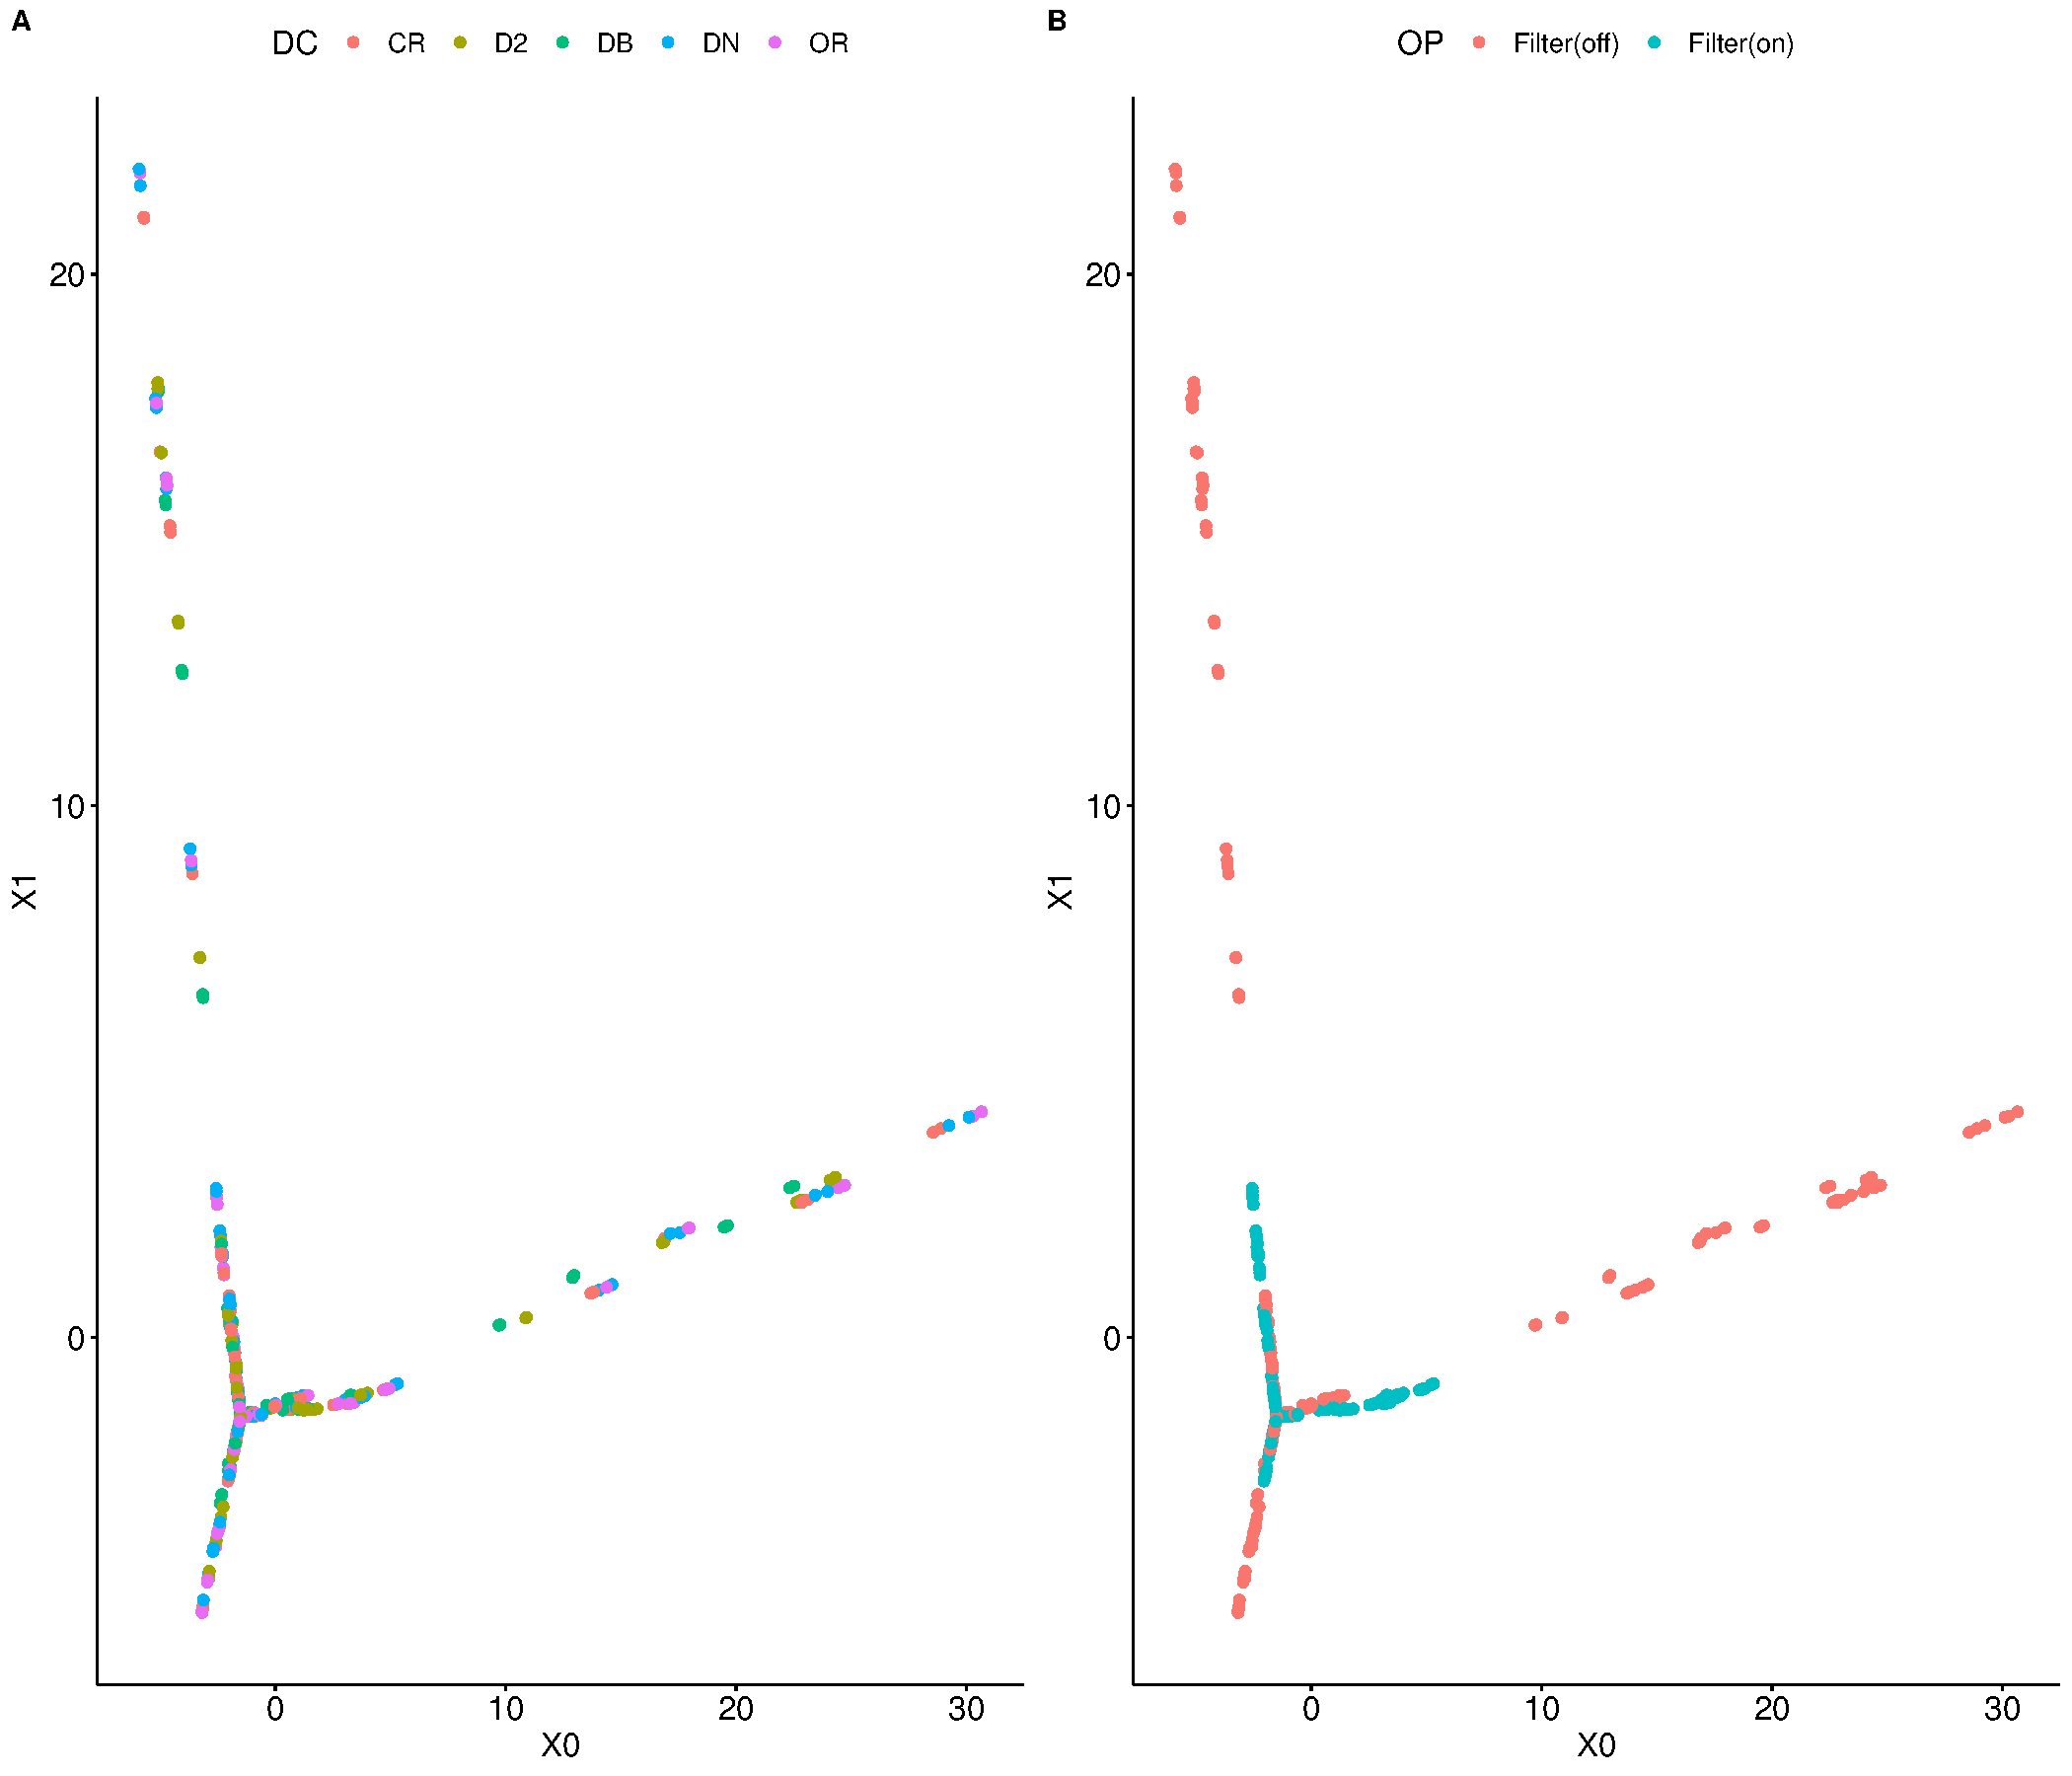
\includegraphics[width=1.0\linewidth]{figure_s1.pdf}
    \end{figure}
    \begin{figure}[H]
      \centering
        \caption{
          \textbf{The variation in the inferred networks in the first two principal axes}
          The plots are colored by the tools or parameters used in the \ac{dc} step (A) and the \ac{op} step (B)
        }
      \label{fig:figure_s1}
    \end{figure}
    \FloatBarrier
    \newpage

    % TODO: Write something about TSNE
    \begin{figure}[H]
      \centering
      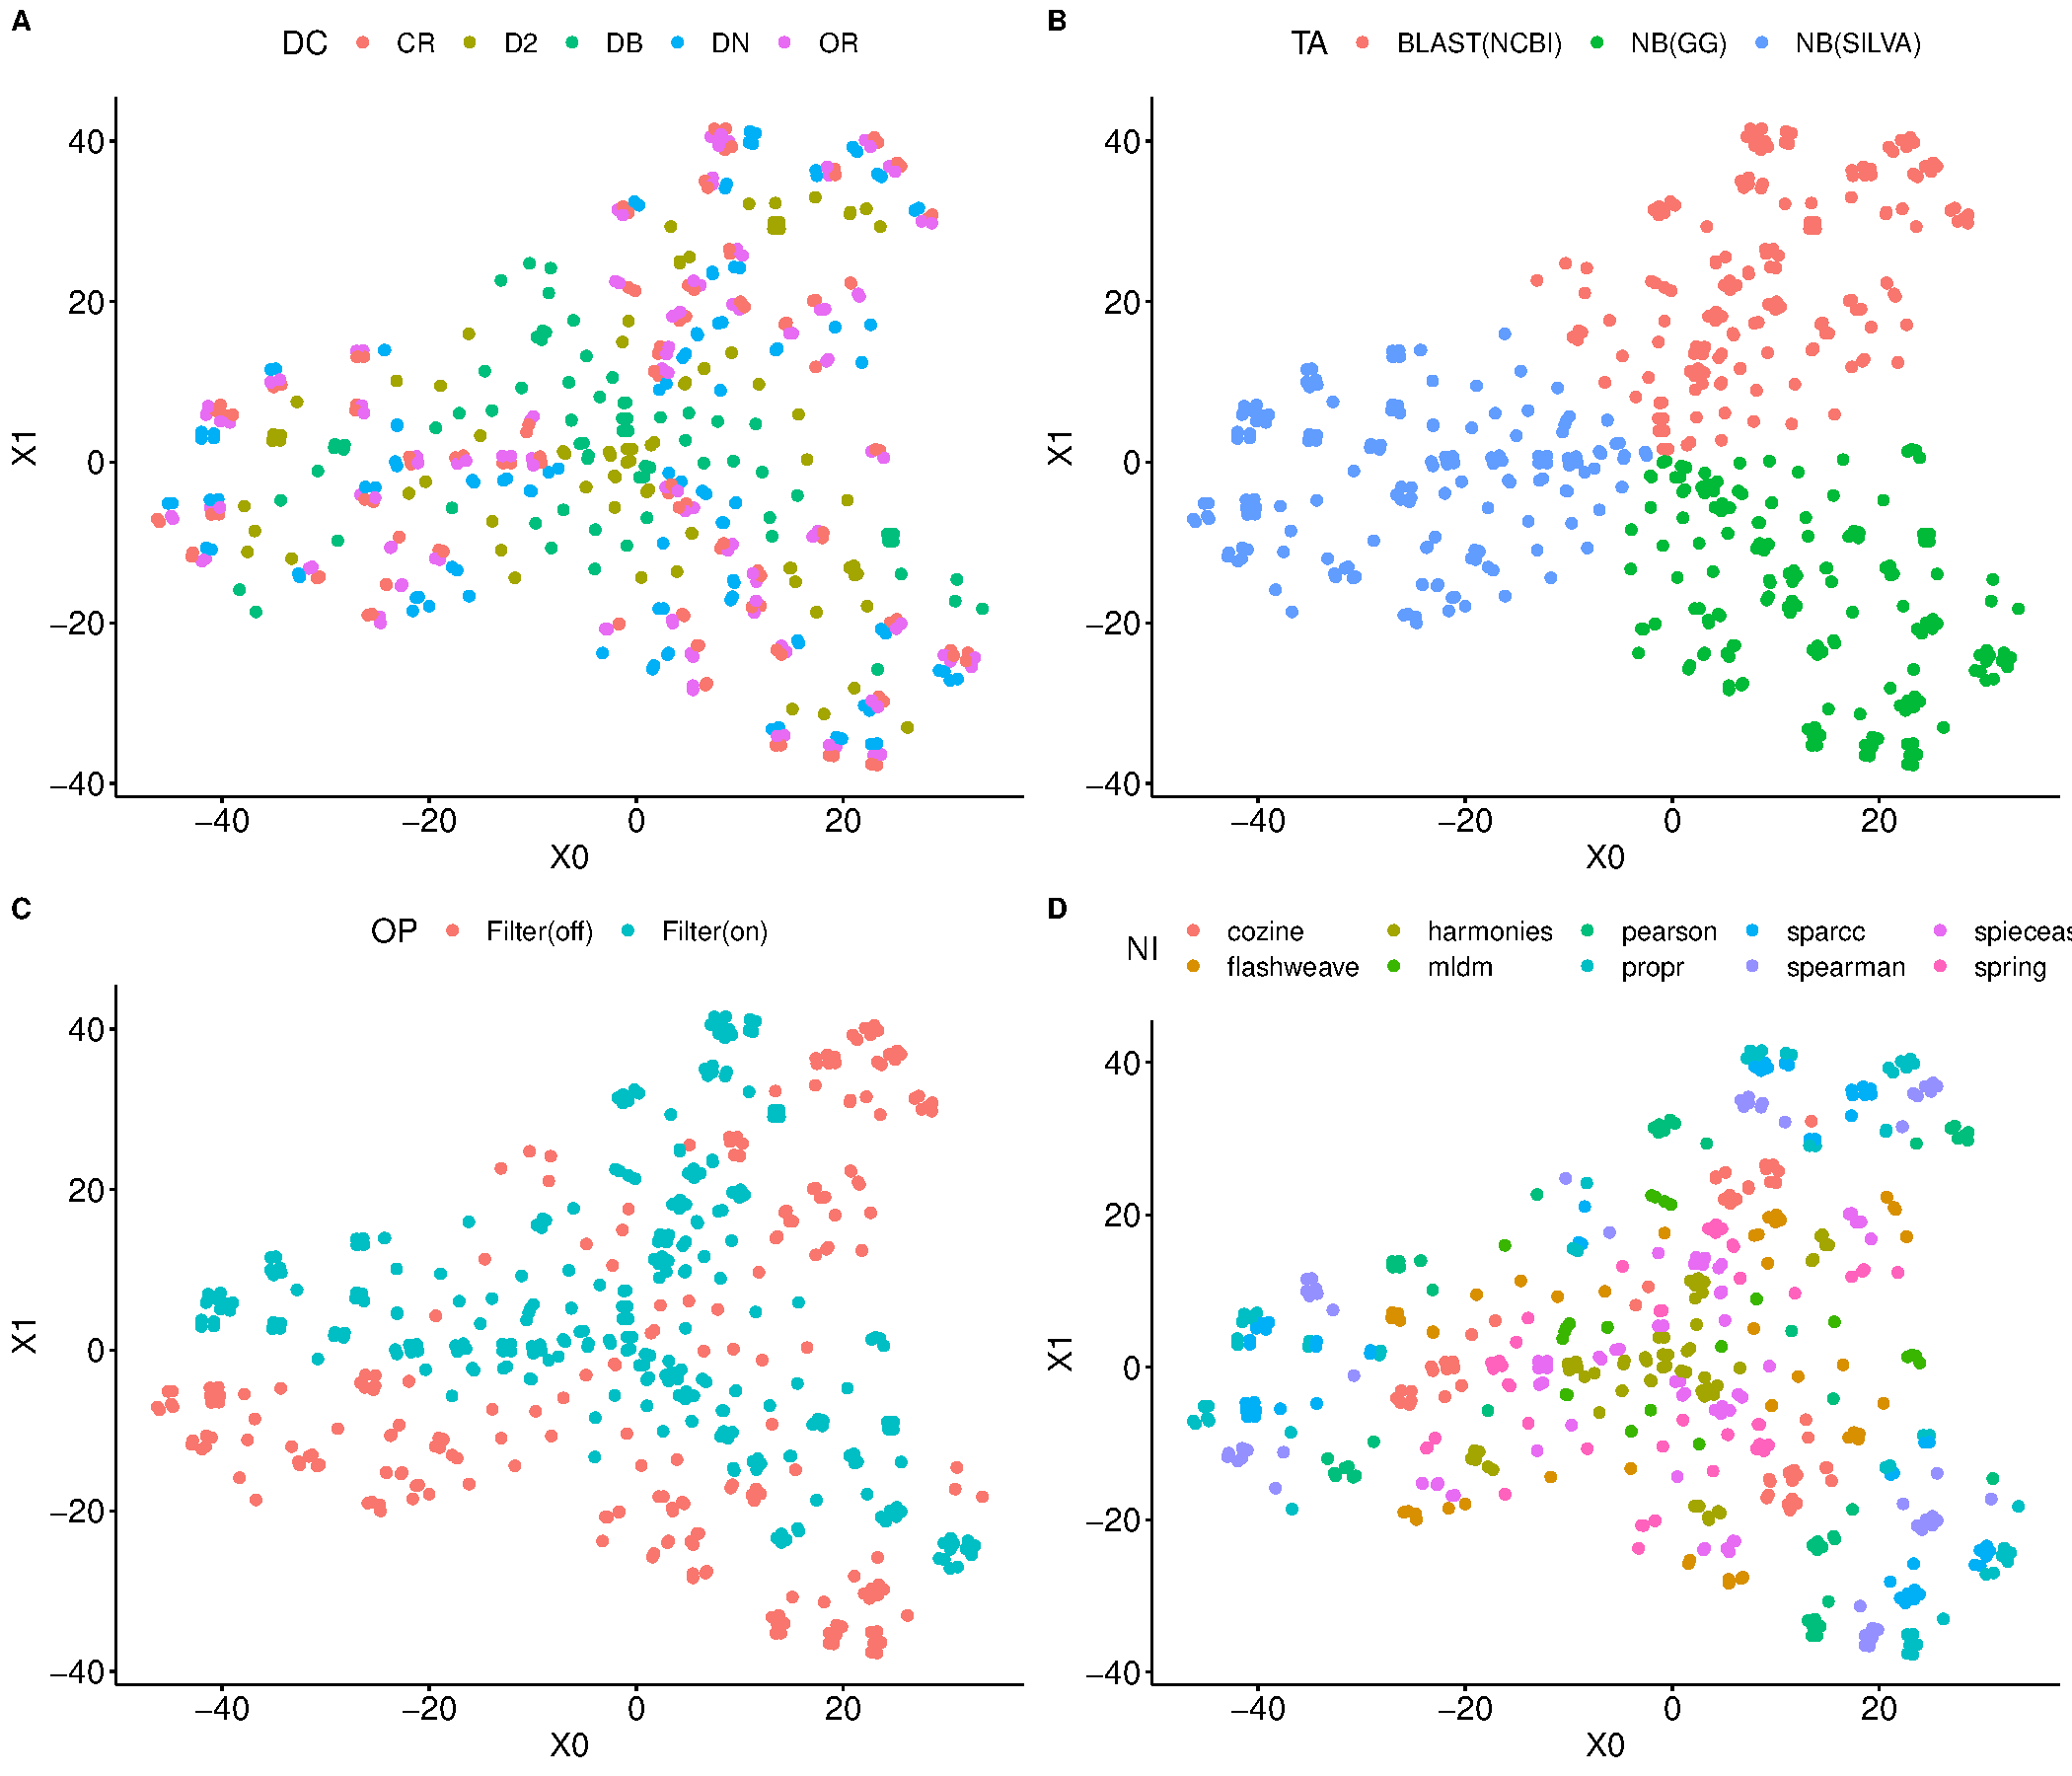
\includegraphics[width=1.0\linewidth]{figure_s2.pdf}
    \end{figure}
    \begin{figure}[H]
      \centering
        \caption{
          \textbf{The TSNE plot of the networks inferred by various methods}.
        }
      \label{fig:figure_s2}
    \end{figure}
    \FloatBarrier
    \newpage

  % QUESTION: Should the CCA section be only included in the response letter?


  \subsection*{Similarity of high abundance reference sequences}

    Figure~\ref{fig:figureS3} is similar to Figure~\ref{fig:figure3} shows the average UniFrac distance between reference sequences generated by the various methods in the \ac{dc} step.
    In Figure~\ref{fig:figureS3} however, we use only the top 1000 representative sequences (by abundance) for this calculation.
    We observe that both the weighted and unweighted UniFrac distances are increased compared to the figure with the all the representative sequences.
    This shows that the most abundant representative sequences generated by the methods are not similar to each other.

    \begin{figure}[H]
      \centering
      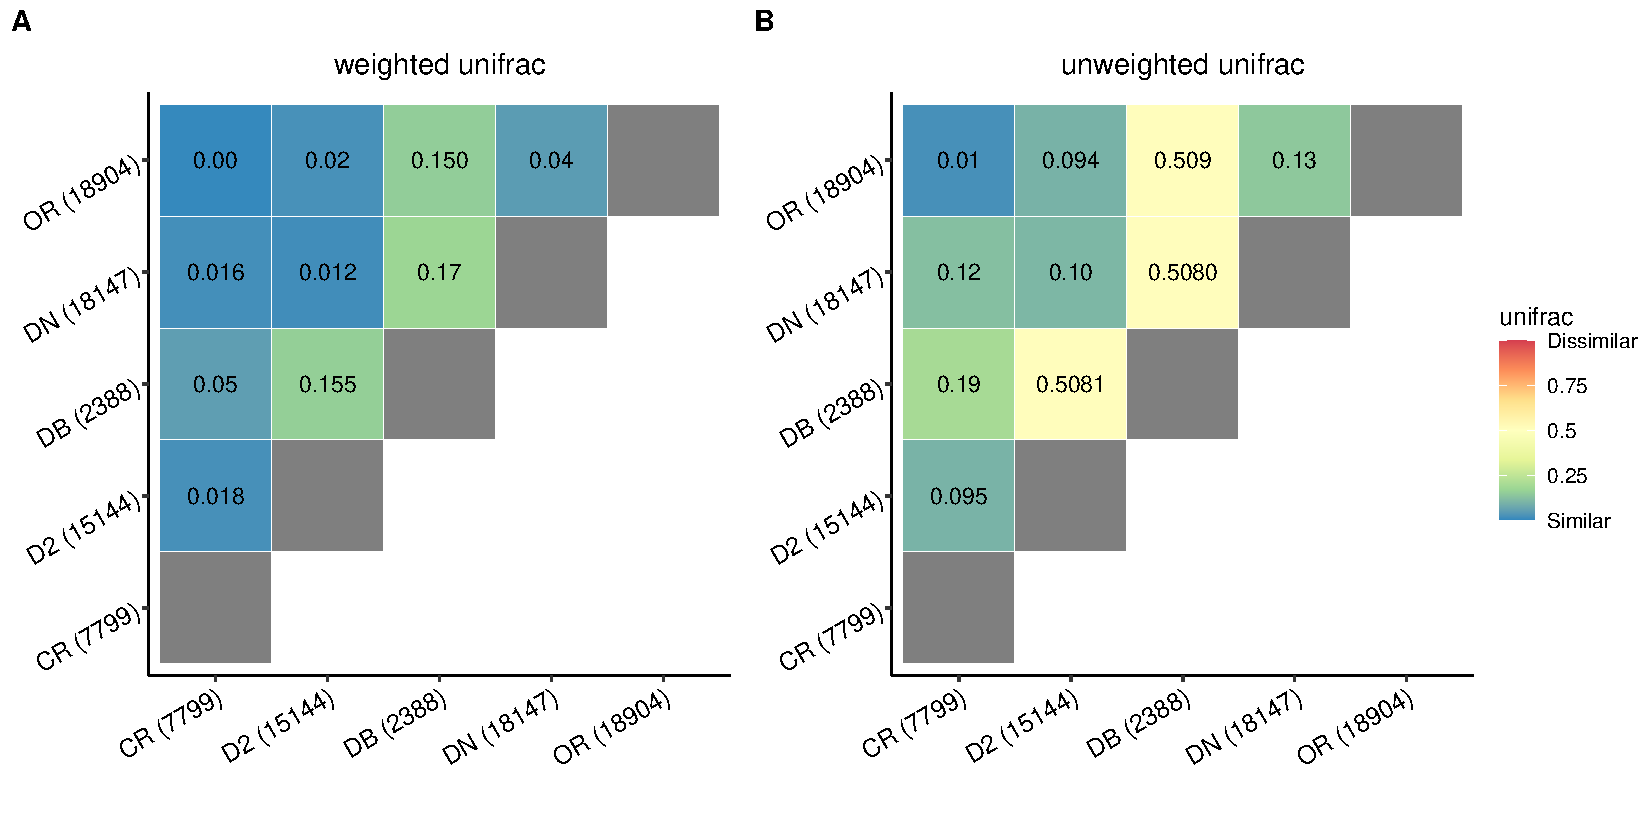
\includegraphics[width=1.0\linewidth]{figure_s3.pdf}
    \end{figure}
    \begin{figure}[H]
      \centering
        \caption{
          \textbf{The UniFrac distance between the 100 most abundant representative sequences generated by various method in the \ac{dc} step}
        }
      \label{fig:figure_s3}
    \end{figure}
    \FloatBarrier
    \newpage

    % TODO: Figure S4 - Unifrac bar plot for CC methods
    \begin{figure}[H]
      \centering
      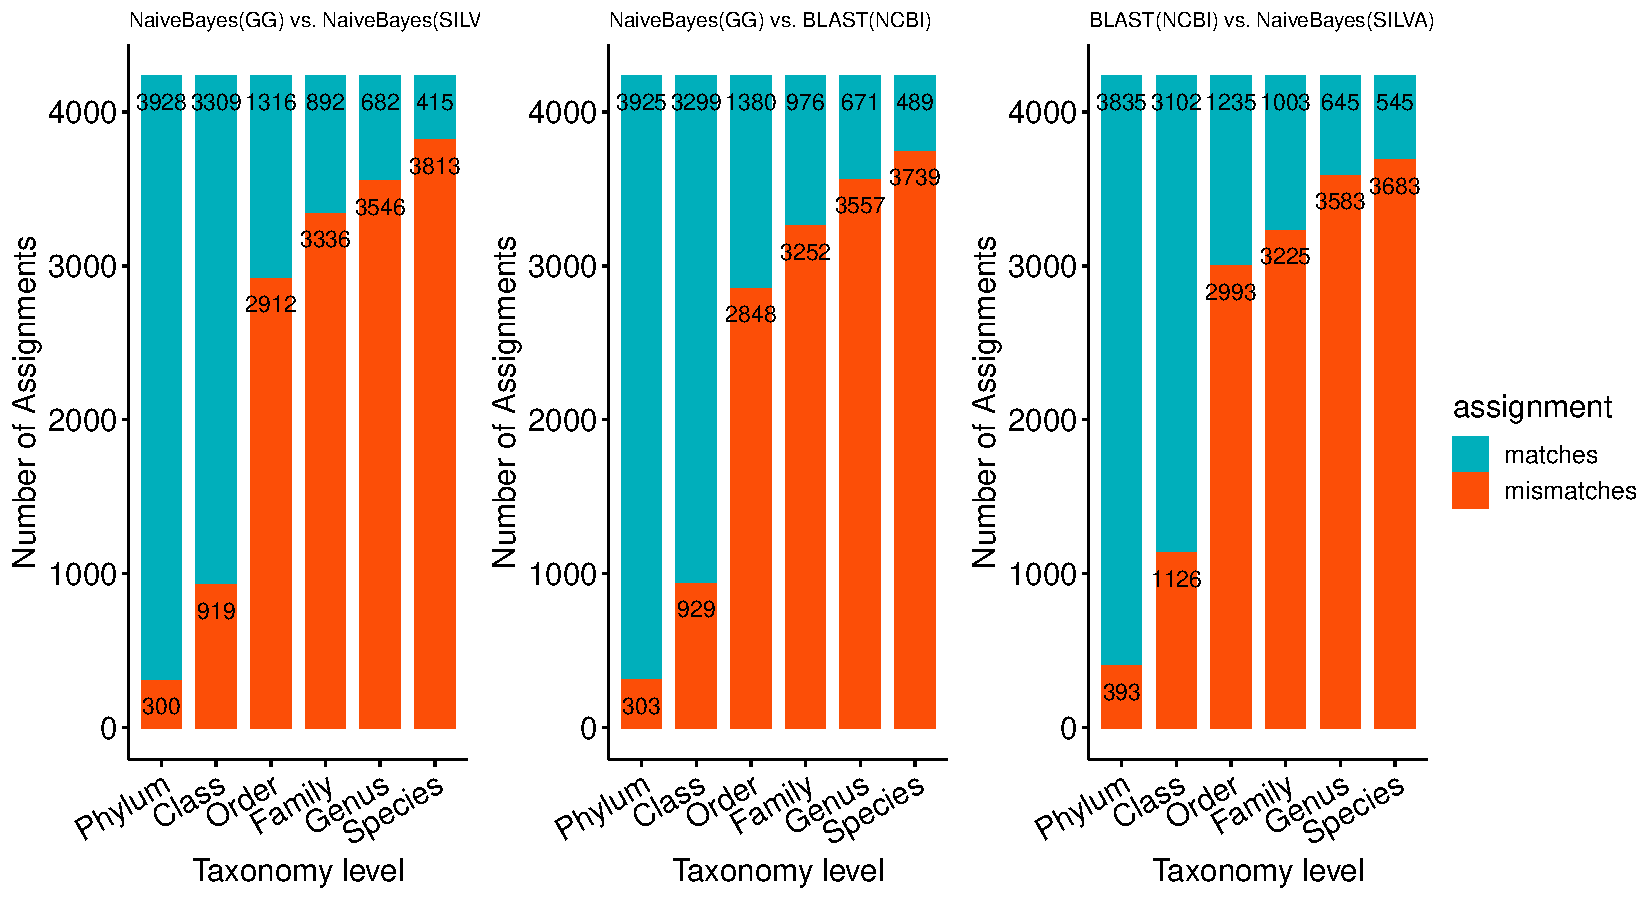
\includegraphics[width=1.0\linewidth]{figure_s4.pdf}
    \end{figure}
    \begin{figure}[H]
      \centering
        \caption{
        }
      \label{fig:figure_s4}
    \end{figure}
    \FloatBarrier
    \newpage

  \subsection*{Mismatches in all assignments at the \ac{TA} step}

    % TODO: Elaborate on this and work on the caption
    Figure~\ref{fig:figure_s5} is similar to Figure~\ref{fig:figure4}B, but instead of the matching only the top 100 taxonomic entities (by abundance), we match all the assignments from one database with those from the other two databases.
    We observe that the percentage of mismatches are indeed higher when considering all the assignments, implying that matching of the taxonomies in the more abundant sequences are more consistent.

    \begin{figure}[H]
      \centering
      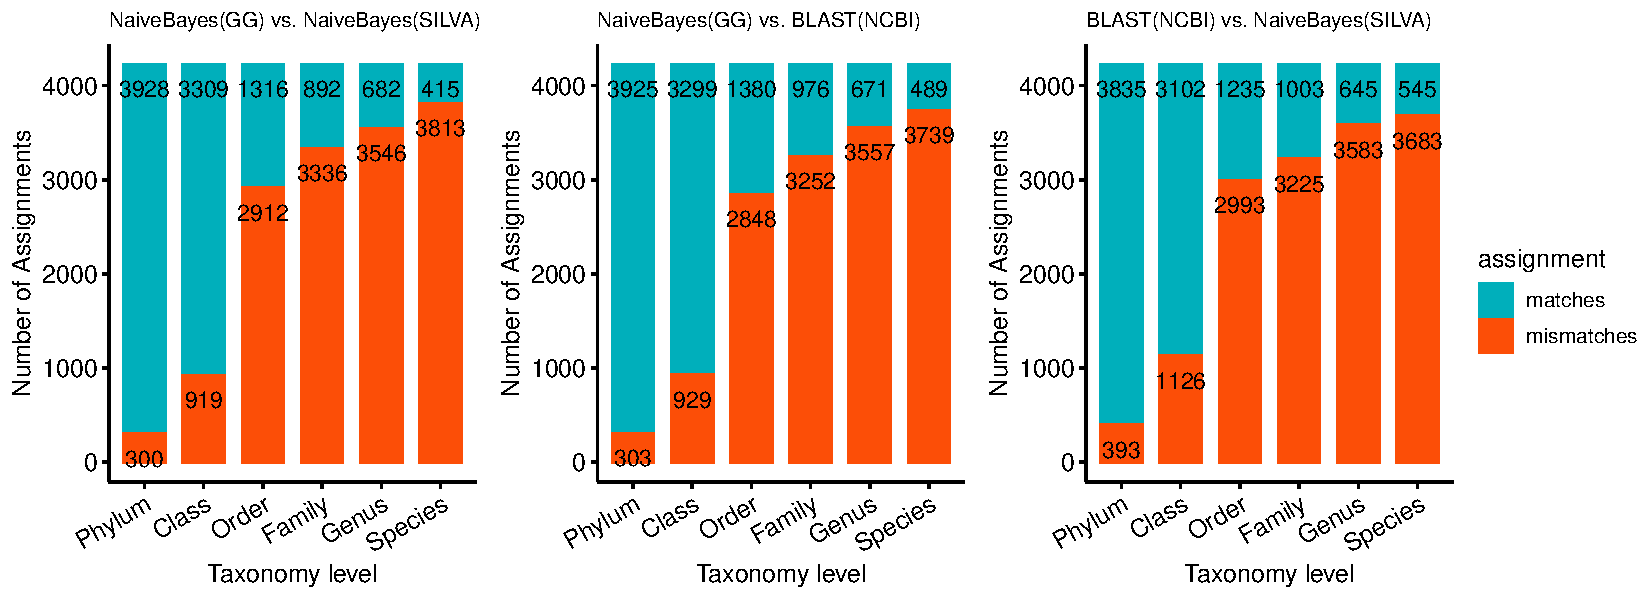
\includegraphics[width=1.0\linewidth]{figure_s5.pdf}
    \end{figure}
    \begin{figure}[H]
      \centering
        \caption{
        }
      \label{fig:figure_s5}
    \end{figure}
    \FloatBarrier
    \newpage

  % TODO: Create table for this section
  % Should this be in the main manuscript?
  \subsection*{Network metrics}

  \subsection*{Consensus and p-value}

  \subsection*{p-value merging}

  Fisher~\cite{fisher_224a_1948} proposed that for $w$ independent p-values, each generated by $w$ different methods and denoted by $\bar{P}^i$, the following will hold true for the statistic $\Psi$:
  \begin{equation*}
    \begin{aligned}
      \Psi &= \sum_{i=1}^w -2 \log \left( \bar{P}^i \right) \\
        \Psi &\sim \chi^2_{2w}
    \end{aligned}
  \end{equation*}

  Brown~\cite{brown_400_1975} extended Fisher's method to dependent p-values by using a re-scaled $\chi^2$ distribution:
  \begin{equation*}
    \Psi \sim c \chi^2_{2f}
  \end{equation*}
  where, $f$ is the degrees of freedom and $c$ is the scale factor and are given by:
  \begin{equation*}
    f = \frac{\mathrm{E}[\Psi]^2}{\mathrm{Var}[\Psi]} ~~~\text{and}~~~ c = \frac{\mathrm{Var}[\Psi]}{2\mathrm{E}[\Psi]} = \frac{w}{f}
  \end{equation*}

  Furthermore, Brown showed that $\mathrm{E}[\Psi]$ and $\mathrm{Var}[\Psi]$ can be calculated via a numerical integration:
  \begin{equation*}
    \mathrm{E}[\Psi] = 2w ~~~\text{and}~~~ \mathrm{Var}[\Psi] = 4w + 2\sum_{i<j} \mathrm{Cov}\left( -2\log(\bar{P}^i), -2\log(\bar{P}^j) \right)
  \end{equation*}

  Kost and McDermott~\cite{kost_combining_2002} further fit a third-order polynomial to approximate the covariance
  \begin{equation}
    \mathrm{Cov}\left( -2\log(\bar{P}^i), -2\log(\bar{P}^j) \right) \approx 3.263 \rho_{ij} + 0.710 \rho_{ij}^2 + 0.027 \rho_{ij}^3
    \label{eqn:covariance-pvalues}
  \end{equation}
  where, $\rho_{ij}$ is the correlation between method $i$ and method $j$

  The final combined p-value~\cite{Poole_Gibbs_Shmulevich_Bernard_Knijnenburg_2016} is then given by:
  \begin{equation}
    \begin{aligned}
        & \hat{P}_j = 1.0 - \Phi_{2f}\left( \psi / c \right) \\
        \text{where},~ &\psi = -2 \sum_{i=1}^w \log(\bar{P}^i_j) ~~~\text{and}~~~ \Phi_{2f} = \mathrm{CDF}\left( \chi^2_{2f} \right)
    \end{aligned}
    \label{eqn:pvalue-combined}
  \end{equation}

  The p-value merging and consensus method in \ac{micone} (refer Documentation) uses Equation~\ref{eqn:covariance-pvalues} to estimate the covariance of the pvalues and Equation~\ref{eqn:pvalue-combined} to merge the p-values (obtained from bootstrapping) from the different correlation methods.
  Note that we do not use Pearson and Spearman methods in the p-value merging step and these algorithms are only used for demonstration and comparison.
  The combined p-values are used to threshold for significance during the consensus network step.

  \subsection*{Performance of alternate consensus network on NorTA data}

    In Figure~\ref{fig:figure_s6} we calculate the consensus network by also taking into account the networks inferred by the Pearson and Spearman methods.
    We see that the consensus networks in this case do not perform as well as those networks that did not incorporate these two algorithms.
    However, we still observe that the consensus network at some parameter values still outperforms the best network inference method (\ac{spieceasi}).

    \begin{figure}[H]
      \centering
      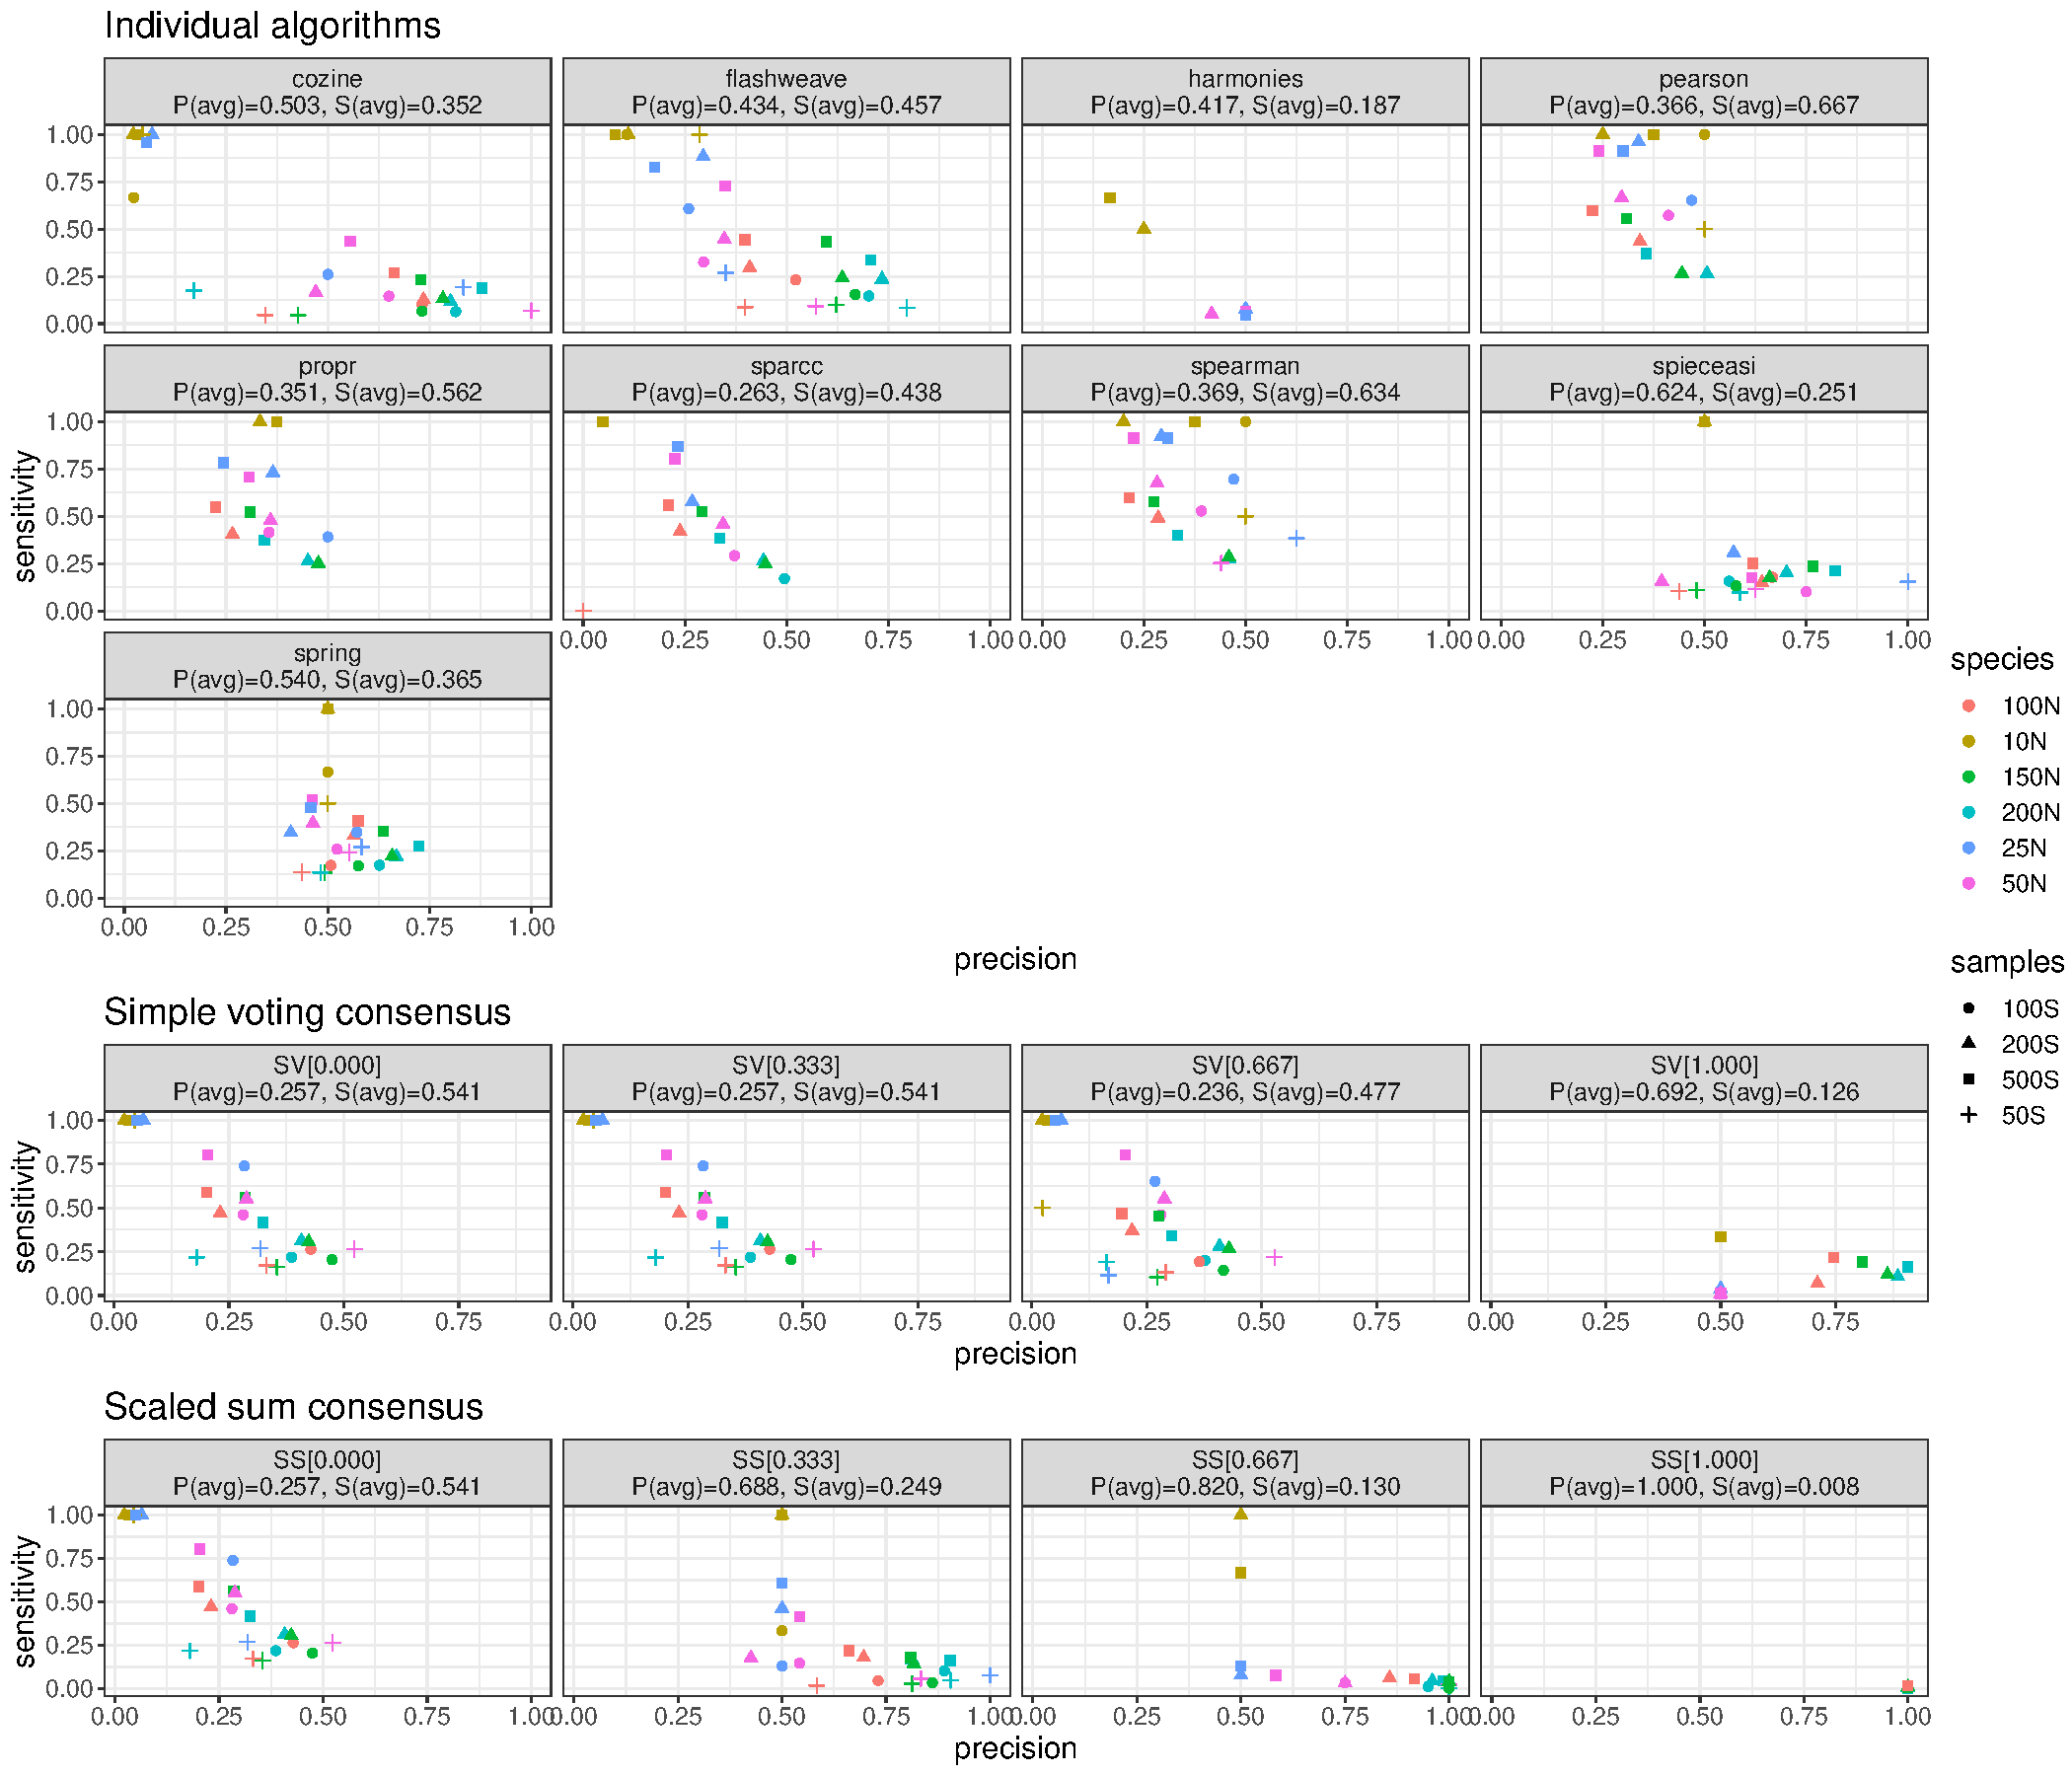
\includegraphics[width=1.0\linewidth]{figure_s6.pdf}
    \end{figure}
    \begin{figure}[H]
      \centering
        \caption{
        }
      \label{fig:figure_s6}
    \end{figure}
    \FloatBarrier
    \newpage


  \subsection*{Performance of network inference algorithms on seqtime data}

    % TODO: Elaborate on this
    In Figure~\ref{fig:figure_s7} we perform the same analysis we did with the NorTA data using the seqtime data.
    We observe that the best performing network inference algorithm is \ac{spieceasi}, but the consensus algorithms, both the scaled-sum and simple voting methods outperform it in terms of precision.
    These results show that the scaled-sum method is much better suited for inferring robust and accurate interactions from count data regardless of the distributions, topologies and number of samples in the data.

    \begin{figure}[H]
      \centering
      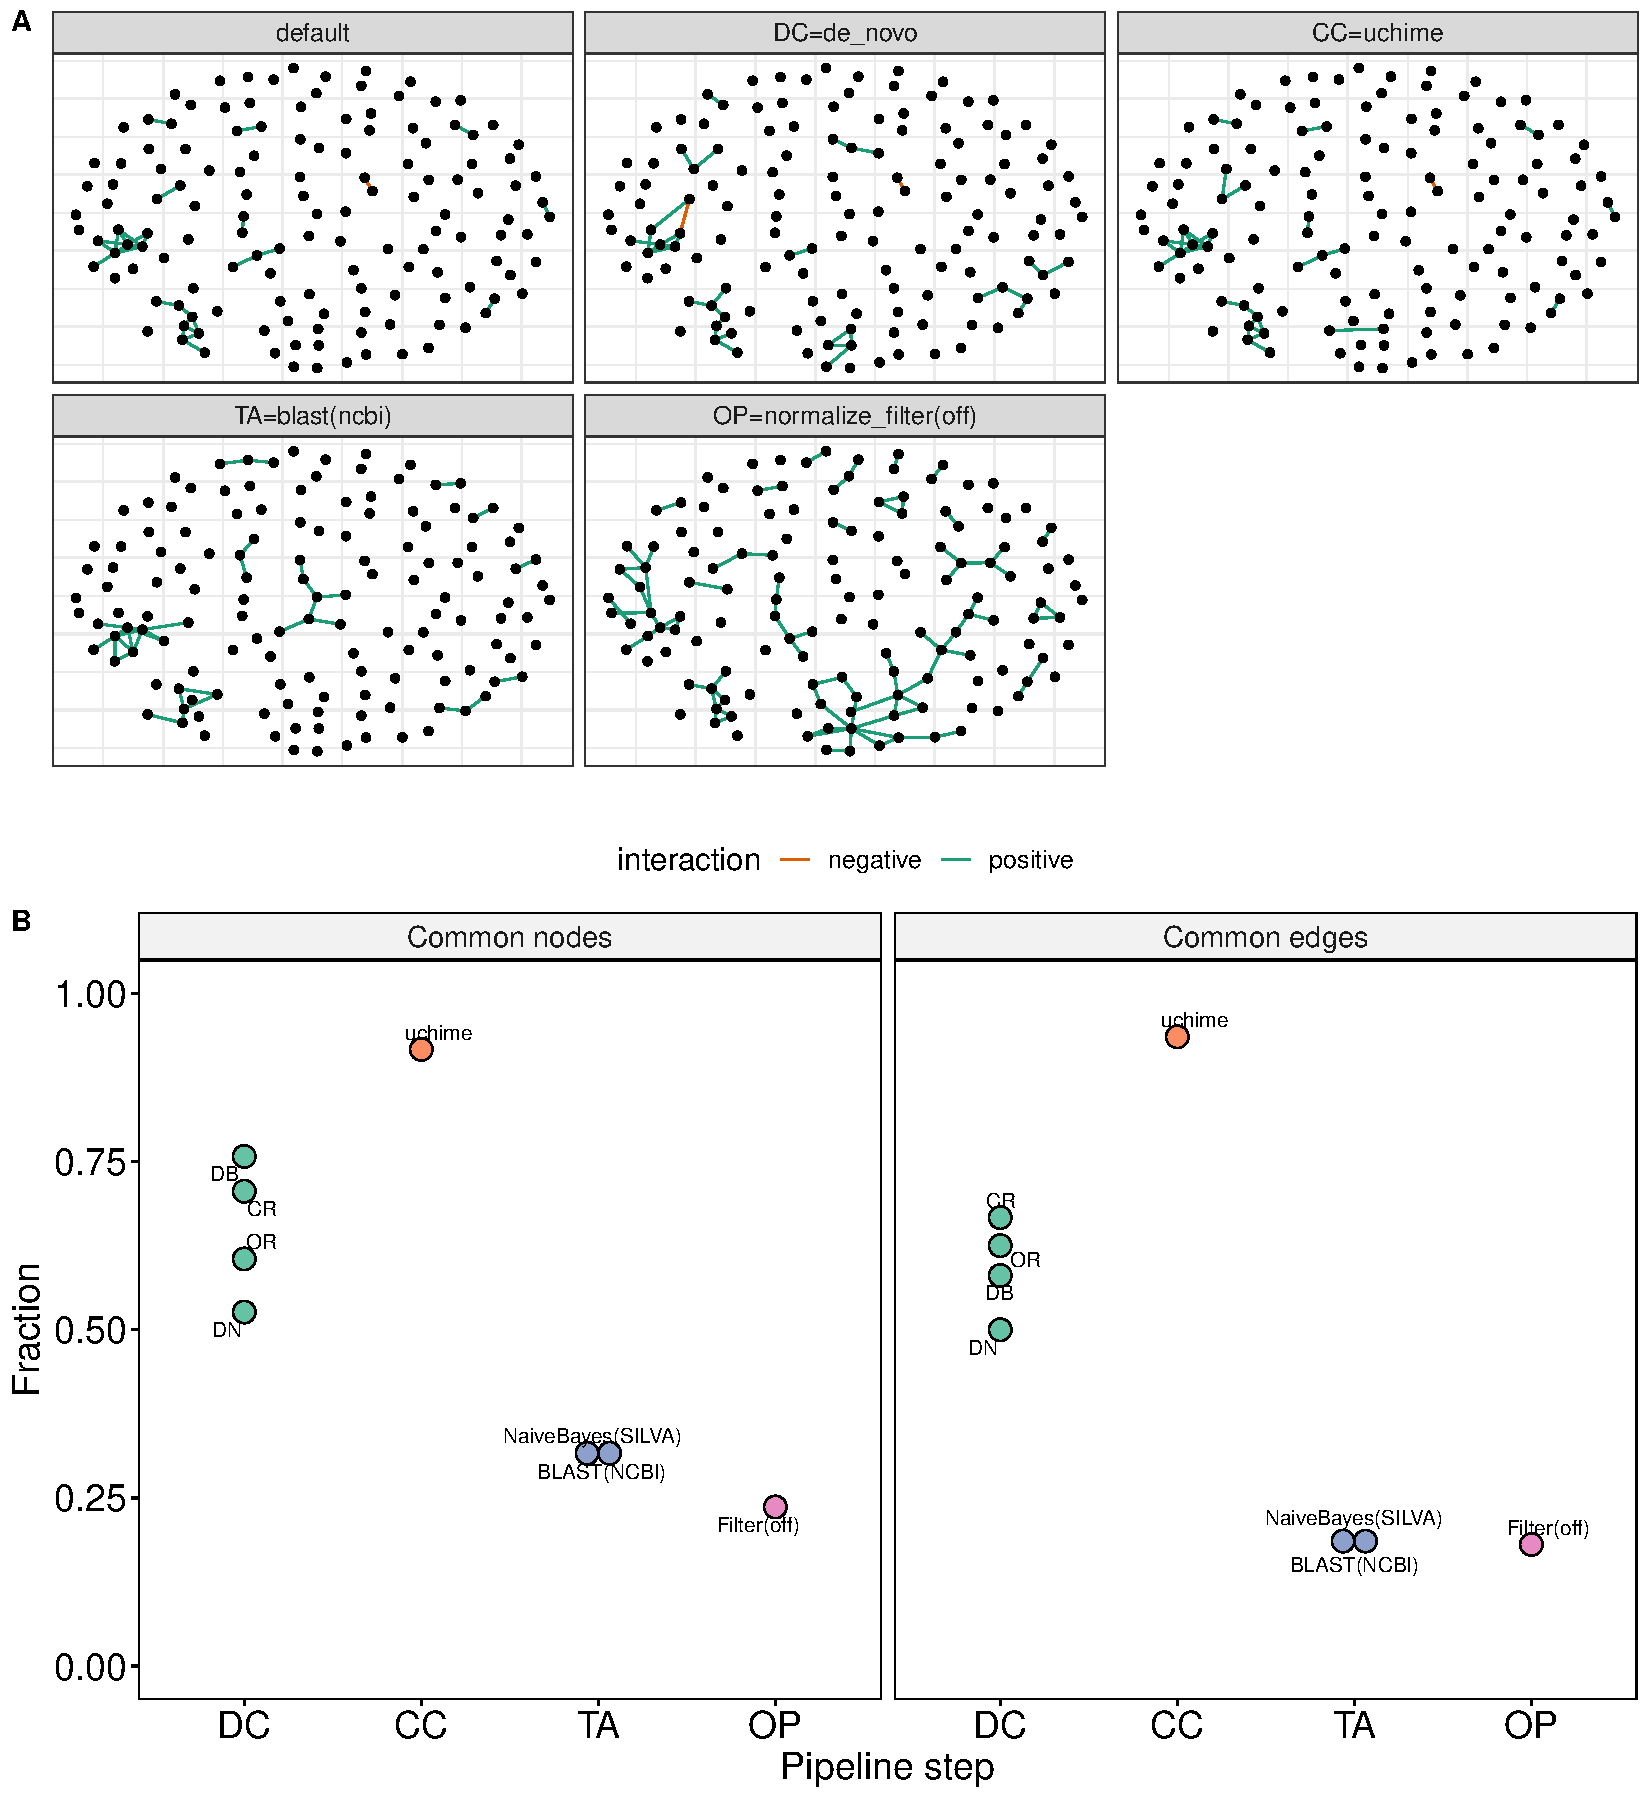
\includegraphics[width=1.0\linewidth]{figure_s7.pdf}
    \end{figure}
    \begin{figure}[H]
      \centering
        \caption{
        }
      \label{fig:figure_s7}
    \end{figure}
    \FloatBarrier
    \newpage


  % TODO: Write more about this and link to documentation
  \subsection*{The JSON network format}

    The default format
